% SOURCE: ../../edit-harness/results/merging_editors/
% !TEX encoding = UTF-8 Unicode
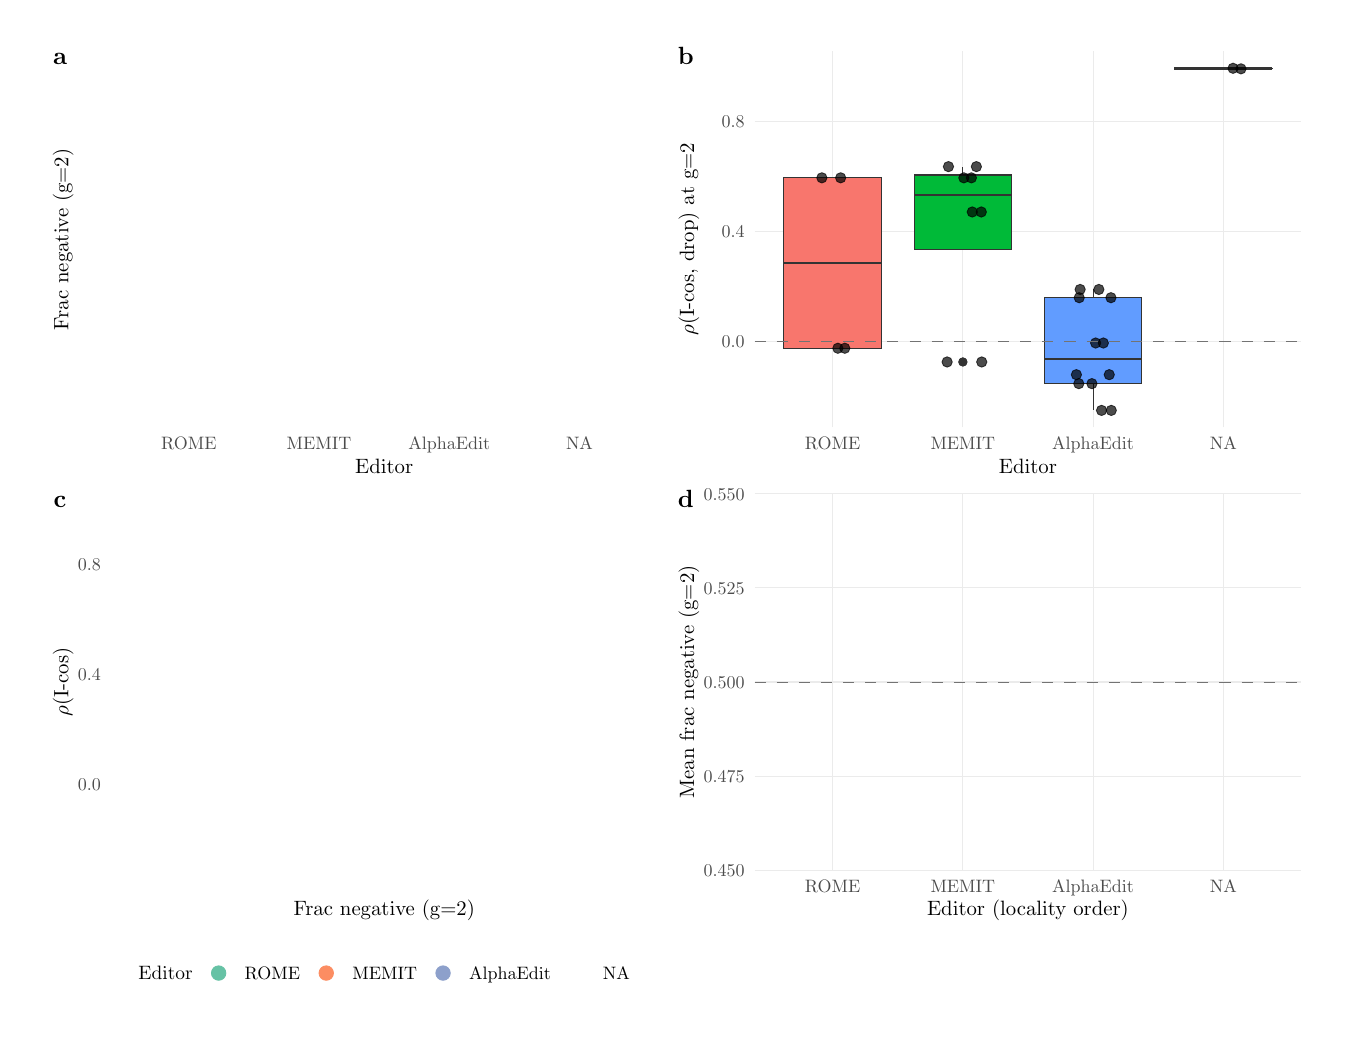
\begin{tikzpicture}[x=1pt,y=1pt]
\definecolor{fillColor}{RGB}{255,255,255}
\path[use as bounding box,fill=fillColor,fill opacity=0.00] (0,0) rectangle (469.75,361.35);
\begin{scope}
\path[clip] (  0.00,  0.00) rectangle (469.75,361.35);
\definecolor{drawColor}{RGB}{255,255,255}
\definecolor{fillColor}{RGB}{255,255,255}

\path[draw=drawColor,line width= 0.6pt,line join=round,line cap=round,fill=fillColor] (  0.00,  0.00) rectangle (469.76,361.35);
\end{scope}
\begin{scope}
\path[clip] (  5.50,195.90) rectangle (231.63,355.85);
\definecolor{fillColor}{RGB}{255,255,255}

\path[fill=fillColor] (  5.50,195.90) rectangle (231.63,355.85);
\end{scope}
\begin{scope}
\path[clip] (231.63,195.90) rectangle (464.26,355.85);
\definecolor{fillColor}{RGB}{255,255,255}

\path[fill=fillColor] (231.63,195.90) rectangle (464.25,355.85);
\end{scope}
\begin{scope}
\path[clip] (  5.50,  5.50) rectangle (231.63,195.90);
\definecolor{fillColor}{RGB}{255,255,255}

\path[fill=fillColor] (  5.50,  5.50) rectangle (231.63,195.90);
\end{scope}
\begin{scope}
\path[clip] (231.63,  5.50) rectangle (464.26,195.90);
\definecolor{fillColor}{RGB}{255,255,255}

\path[fill=fillColor] (231.63,  5.50) rectangle (464.25,195.90);
\end{scope}
\begin{scope}
\path[clip] (  0.00,  0.00) rectangle (469.75,361.35);
\definecolor{drawColor}{gray}{0.30}

\node[text=drawColor,anchor=base,inner sep=0pt, outer sep=0pt, scale=  0.65] at ( 58.26,208.79) {ROME};

\node[text=drawColor,anchor=base,inner sep=0pt, outer sep=0pt, scale=  0.65] at (105.30,208.79) {MEMIT};

\node[text=drawColor,anchor=base,inner sep=0pt, outer sep=0pt, scale=  0.65] at (152.35,208.79) {AlphaEdit};

\node[text=drawColor,anchor=base,inner sep=0pt, outer sep=0pt, scale=  0.65] at (199.40,208.79) {NA};
\end{scope}
\begin{scope}
\path[clip] (  0.00,  0.00) rectangle (469.75,361.35);
\definecolor{drawColor}{RGB}{0,0,0}

\node[text=drawColor,anchor=base,inner sep=0pt, outer sep=0pt, scale=  0.75] at (128.83,200.36) {Editor};
\end{scope}
\begin{scope}
\path[clip] (  0.00,  0.00) rectangle (469.75,361.35);
\definecolor{drawColor}{RGB}{0,0,0}

\node[text=drawColor,rotate= 90.00,anchor=base,inner sep=0pt, outer sep=0pt, scale=  0.75] at ( 14.67,284.86) {Frac negative (g=2)};
\end{scope}
\begin{scope}
\path[clip] (  0.00,  0.00) rectangle (469.75,361.35);
\definecolor{drawColor}{RGB}{0,0,0}

\node[text=drawColor,anchor=base,inner sep=0pt, outer sep=0pt, scale=  0.90] at ( 11.68,348.21) {\bfseries a};
\end{scope}
\begin{scope}
\path[clip] (262.65,216.87) rectangle (460.25,352.85);
\definecolor{drawColor}{gray}{0.92}

\path[draw=drawColor,line width= 0.4pt,line join=round] (262.65,248.02) --
	(460.25,248.02);

\path[draw=drawColor,line width= 0.4pt,line join=round] (262.65,287.70) --
	(460.25,287.70);

\path[draw=drawColor,line width= 0.4pt,line join=round] (262.65,327.38) --
	(460.25,327.38);

\path[draw=drawColor,line width= 0.4pt,line join=round] (290.88,216.87) --
	(290.88,352.85);

\path[draw=drawColor,line width= 0.4pt,line join=round] (337.93,216.87) --
	(337.93,352.85);

\path[draw=drawColor,line width= 0.4pt,line join=round] (384.98,216.87) --
	(384.98,352.85);

\path[draw=drawColor,line width= 0.4pt,line join=round] (432.03,216.87) --
	(432.03,352.85);
\definecolor{drawColor}{gray}{0.20}

\path[draw=drawColor,line width= 0.4pt,line join=round] (290.88,307.09) -- (290.88,307.09);

\path[draw=drawColor,line width= 0.4pt,line join=round] (290.88,245.51) -- (290.88,245.51);
\definecolor{fillColor}{RGB}{248,118,109}

\path[draw=drawColor,line width= 0.4pt,fill=fillColor] (273.24,307.09) --
	(273.24,245.51) --
	(308.53,245.51) --
	(308.53,307.09) --
	(273.24,307.09) --
	cycle;

\path[draw=drawColor,line width= 0.8pt] (273.24,276.30) -- (308.53,276.30);
\definecolor{fillColor}{gray}{0.20}

\path[draw=drawColor,line width= 0.4pt,line join=round,line cap=round,fill=fillColor] (337.93,240.55) circle (  1.43);

\path[draw=drawColor,line width= 0.4pt,line join=round,line cap=round,fill=fillColor] (337.93,240.55) circle (  1.43);

\path[draw=drawColor,line width= 0.4pt,line join=round] (337.93,308.09) -- (337.93,311.13);

\path[draw=drawColor,line width= 0.4pt,line join=round] (337.93,281.20) -- (337.93,281.20);
\definecolor{fillColor}{RGB}{0,186,56}

\path[draw=drawColor,line width= 0.4pt,fill=fillColor] (320.29,308.09) --
	(320.29,281.20) --
	(355.57,281.20) --
	(355.57,308.09) --
	(320.29,308.09) --
	cycle;

\path[draw=drawColor,line width= 0.8pt] (320.29,300.91) -- (355.57,300.91);

\path[draw=drawColor,line width= 0.4pt,line join=round] (384.98,263.77) -- (384.98,266.75);

\path[draw=drawColor,line width= 0.4pt,line join=round] (384.98,232.72) -- (384.98,223.05);
\definecolor{fillColor}{RGB}{97,156,255}

\path[draw=drawColor,line width= 0.4pt,fill=fillColor] (367.34,263.77) --
	(367.34,232.72) --
	(402.62,232.72) --
	(402.62,263.77) --
	(367.34,263.77) --
	cycle;

\path[draw=drawColor,line width= 0.8pt] (367.34,241.68) -- (402.62,241.68);

\path[draw=drawColor,line width= 0.4pt,line join=round] (432.03,346.62) -- (432.03,346.67);

\path[draw=drawColor,line width= 0.4pt,line join=round] (432.03,346.52) -- (432.03,346.47);
\definecolor{fillColor}{gray}{0.50}

\path[draw=drawColor,line width= 0.4pt,fill=fillColor] (414.38,346.62) --
	(414.38,346.52) --
	(449.67,346.52) --
	(449.67,346.62) --
	(414.38,346.62) --
	cycle;

\path[draw=drawColor,line width= 0.8pt] (414.38,346.57) -- (449.67,346.57);
\definecolor{drawColor}{RGB}{0,0,0}
\definecolor{fillColor}{RGB}{0,0,0}

\path[draw=drawColor,draw opacity=0.70,line width= 0.3pt,line join=round,line cap=round,fill=fillColor,fill opacity=0.70] (378.95,235.96) circle (  1.87);

\path[draw=drawColor,draw opacity=0.70,line width= 0.3pt,line join=round,line cap=round,fill=fillColor,fill opacity=0.70] (387.07,266.75) circle (  1.87);

\path[draw=drawColor,draw opacity=0.70,line width= 0.3pt,line join=round,line cap=round,fill=fillColor,fill opacity=0.70] (341.32,294.75) circle (  1.87);

\path[draw=drawColor,draw opacity=0.70,line width= 0.3pt,line join=round,line cap=round,fill=fillColor,fill opacity=0.70] (379.97,263.77) circle (  1.87);

\path[draw=drawColor,draw opacity=0.70,line width= 0.3pt,line join=round,line cap=round,fill=fillColor,fill opacity=0.70] (342.81,311.13) circle (  1.87);

\path[draw=drawColor,draw opacity=0.70,line width= 0.3pt,line join=round,line cap=round,fill=fillColor,fill opacity=0.70] (293.77,307.09) circle (  1.87);

\path[draw=drawColor,draw opacity=0.70,line width= 0.3pt,line join=round,line cap=round,fill=fillColor,fill opacity=0.70] (341.01,307.08) circle (  1.87);

\path[draw=drawColor,draw opacity=0.70,line width= 0.3pt,line join=round,line cap=round,fill=fillColor,fill opacity=0.70] (379.82,232.72) circle (  1.87);

\path[draw=drawColor,draw opacity=0.70,line width= 0.3pt,line join=round,line cap=round,fill=fillColor,fill opacity=0.70] (385.91,247.40) circle (  1.87);

\path[draw=drawColor,draw opacity=0.70,line width= 0.3pt,line join=round,line cap=round,fill=fillColor,fill opacity=0.70] (344.75,240.55) circle (  1.87);

\path[draw=drawColor,draw opacity=0.70,line width= 0.3pt,line join=round,line cap=round,fill=fillColor,fill opacity=0.70] (292.76,245.51) circle (  1.87);

\path[draw=drawColor,draw opacity=0.70,line width= 0.3pt,line join=round,line cap=round,fill=fillColor,fill opacity=0.70] (388.04,223.05) circle (  1.87);

\path[draw=drawColor,draw opacity=0.70,line width= 0.3pt,line join=round,line cap=round,fill=fillColor,fill opacity=0.70] (390.82,235.96) circle (  1.87);

\path[draw=drawColor,draw opacity=0.70,line width= 0.3pt,line join=round,line cap=round,fill=fillColor,fill opacity=0.70] (391.44,263.77) circle (  1.87);

\path[draw=drawColor,draw opacity=0.70,line width= 0.3pt,line join=round,line cap=round,fill=fillColor,fill opacity=0.70] (332.72,311.13) circle (  1.87);

\path[draw=drawColor,draw opacity=0.70,line width= 0.3pt,line join=round,line cap=round,fill=fillColor,fill opacity=0.70] (286.98,307.09) circle (  1.87);

\path[draw=drawColor,draw opacity=0.70,line width= 0.3pt,line join=round,line cap=round,fill=fillColor,fill opacity=0.70] (338.28,307.08) circle (  1.87);

\path[draw=drawColor,draw opacity=0.70,line width= 0.3pt,line join=round,line cap=round,fill=fillColor,fill opacity=0.70] (380.30,266.75) circle (  1.87);

\path[draw=drawColor,draw opacity=0.70,line width= 0.3pt,line join=round,line cap=round,fill=fillColor,fill opacity=0.70] (344.59,294.75) circle (  1.87);

\path[draw=drawColor,draw opacity=0.70,line width= 0.3pt,line join=round,line cap=round,fill=fillColor,fill opacity=0.70] (384.56,232.72) circle (  1.87);

\path[draw=drawColor,draw opacity=0.70,line width= 0.3pt,line join=round,line cap=round,fill=fillColor,fill opacity=0.70] (391.55,223.05) circle (  1.87);

\path[draw=drawColor,draw opacity=0.70,line width= 0.3pt,line join=round,line cap=round,fill=fillColor,fill opacity=0.70] (388.69,247.40) circle (  1.87);

\path[draw=drawColor,draw opacity=0.70,line width= 0.3pt,line join=round,line cap=round,fill=fillColor,fill opacity=0.70] (332.24,240.55) circle (  1.87);

\path[draw=drawColor,draw opacity=0.70,line width= 0.3pt,line join=round,line cap=round,fill=fillColor,fill opacity=0.70] (295.26,245.51) circle (  1.87);

\path[draw=drawColor,draw opacity=0.70,line width= 0.3pt,line join=round,line cap=round,fill=fillColor,fill opacity=0.70] (435.56,346.67) circle (  1.87);

\path[draw=drawColor,draw opacity=0.70,line width= 0.3pt,line join=round,line cap=round,fill=fillColor,fill opacity=0.70] (438.42,346.47) circle (  1.87);
\definecolor{drawColor}{gray}{0.45}

\path[draw=drawColor,line width= 0.3pt,dash pattern=on 4pt off 4pt ,line join=round] (262.65,248.02) -- (460.25,248.02);
\end{scope}
\begin{scope}
\path[clip] (  0.00,  0.00) rectangle (469.75,361.35);
\definecolor{drawColor}{gray}{0.30}

\node[text=drawColor,anchor=base east,inner sep=0pt, outer sep=0pt, scale=  0.65] at (259.05,245.79) {0.0};

\node[text=drawColor,anchor=base east,inner sep=0pt, outer sep=0pt, scale=  0.65] at (259.05,285.46) {0.4};

\node[text=drawColor,anchor=base east,inner sep=0pt, outer sep=0pt, scale=  0.65] at (259.05,325.14) {0.8};
\end{scope}
\begin{scope}
\path[clip] (  0.00,  0.00) rectangle (469.75,361.35);
\definecolor{drawColor}{gray}{0.30}

\node[text=drawColor,anchor=base,inner sep=0pt, outer sep=0pt, scale=  0.65] at (290.88,208.79) {ROME};

\node[text=drawColor,anchor=base,inner sep=0pt, outer sep=0pt, scale=  0.65] at (337.93,208.79) {MEMIT};

\node[text=drawColor,anchor=base,inner sep=0pt, outer sep=0pt, scale=  0.65] at (384.98,208.79) {AlphaEdit};

\node[text=drawColor,anchor=base,inner sep=0pt, outer sep=0pt, scale=  0.65] at (432.03,208.79) {NA};
\end{scope}
\begin{scope}
\path[clip] (  0.00,  0.00) rectangle (469.75,361.35);
\definecolor{drawColor}{RGB}{0,0,0}

\node[text=drawColor,anchor=base,inner sep=0pt, outer sep=0pt, scale=  0.75] at (361.45,200.36) {Editor};
\end{scope}
\begin{scope}
\path[clip] (  0.00,  0.00) rectangle (469.75,361.35);
\definecolor{drawColor}{RGB}{0,0,0}

\node[text=drawColor,rotate= 90.00,anchor=base,inner sep=0pt, outer sep=0pt, scale=  0.75] at (240.79,284.86) {$\rho$(I-cos, drop) at g=2};
\end{scope}
\begin{scope}
\path[clip] (  0.00,  0.00) rectangle (469.75,361.35);
\definecolor{drawColor}{RGB}{0,0,0}

\node[text=drawColor,anchor=base,inner sep=0pt, outer sep=0pt, scale=  0.90] at (237.87,348.21) {\bfseries b};
\end{scope}
\begin{scope}
\path[clip] (  0.00,  0.00) rectangle (469.75,361.35);
\definecolor{drawColor}{gray}{0.30}

\node[text=drawColor,anchor=base east,inner sep=0pt, outer sep=0pt, scale=  0.65] at ( 26.43, 85.84) {0.0};

\node[text=drawColor,anchor=base east,inner sep=0pt, outer sep=0pt, scale=  0.65] at ( 26.43,125.51) {0.4};

\node[text=drawColor,anchor=base east,inner sep=0pt, outer sep=0pt, scale=  0.65] at ( 26.43,165.19) {0.8};
\end{scope}
\begin{scope}
\path[clip] (  0.00,  0.00) rectangle (469.75,361.35);
\definecolor{drawColor}{RGB}{0,0,0}

\node[text=drawColor,anchor=base,inner sep=0pt, outer sep=0pt, scale=  0.75] at (128.83, 40.41) {Frac negative (g=2)};
\end{scope}
\begin{scope}
\path[clip] (  0.00,  0.00) rectangle (469.75,361.35);
\definecolor{drawColor}{RGB}{0,0,0}

\node[text=drawColor,rotate= 90.00,anchor=base,inner sep=0pt, outer sep=0pt, scale=  0.75] at ( 14.67,124.91) {$\rho$(I-cos)};
\end{scope}
\begin{scope}
\path[clip] (  0.00,  0.00) rectangle (469.75,361.35);
\definecolor{drawColor}{RGB}{0,0,0}

\node[text=drawColor,anchor=base west,inner sep=0pt, outer sep=0pt, scale=  0.70] at ( 40.03, 17.32) {Editor};
\end{scope}
\begin{scope}
\path[clip] (  0.00,  0.00) rectangle (469.75,361.35);
\definecolor{drawColor}{RGB}{102,194,165}
\definecolor{fillColor}{RGB}{102,194,165}

\path[draw=drawColor,line width= 0.3pt,line join=round,line cap=round,fill=fillColor] ( 69.01, 19.73) circle (  2.61);
\end{scope}
\begin{scope}
\path[clip] (  0.00,  0.00) rectangle (469.75,361.35);
\definecolor{drawColor}{RGB}{252,141,98}
\definecolor{fillColor}{RGB}{252,141,98}

\path[draw=drawColor,line width= 0.3pt,line join=round,line cap=round,fill=fillColor] (107.89, 19.73) circle (  2.61);
\end{scope}
\begin{scope}
\path[clip] (  0.00,  0.00) rectangle (469.75,361.35);
\definecolor{drawColor}{RGB}{141,160,203}
\definecolor{fillColor}{RGB}{141,160,203}

\path[draw=drawColor,line width= 0.3pt,line join=round,line cap=round,fill=fillColor] (150.10, 19.73) circle (  2.61);
\end{scope}
\begin{scope}
\path[clip] (  0.00,  0.00) rectangle (469.75,361.35);

\path[] (198.46, 19.73) circle (  2.61);
\end{scope}
\begin{scope}
\path[clip] (  0.00,  0.00) rectangle (469.75,361.35);
\definecolor{drawColor}{RGB}{0,0,0}

\node[text=drawColor,anchor=base west,inner sep=0pt, outer sep=0pt, scale=  0.65] at ( 78.43, 17.49) {ROME};
\end{scope}
\begin{scope}
\path[clip] (  0.00,  0.00) rectangle (469.75,361.35);
\definecolor{drawColor}{RGB}{0,0,0}

\node[text=drawColor,anchor=base west,inner sep=0pt, outer sep=0pt, scale=  0.65] at (117.31, 17.49) {MEMIT};
\end{scope}
\begin{scope}
\path[clip] (  0.00,  0.00) rectangle (469.75,361.35);
\definecolor{drawColor}{RGB}{0,0,0}

\node[text=drawColor,anchor=base west,inner sep=0pt, outer sep=0pt, scale=  0.65] at (159.52, 17.49) {AlphaEdit};
\end{scope}
\begin{scope}
\path[clip] (  0.00,  0.00) rectangle (469.75,361.35);
\definecolor{drawColor}{RGB}{0,0,0}

\node[text=drawColor,anchor=base west,inner sep=0pt, outer sep=0pt, scale=  0.65] at (207.88, 17.49) {NA};
\end{scope}
\begin{scope}
\path[clip] (  0.00,  0.00) rectangle (469.75,361.35);
\definecolor{drawColor}{RGB}{0,0,0}

\node[text=drawColor,anchor=base,inner sep=0pt, outer sep=0pt, scale=  0.90] at ( 11.68,187.95) {\bfseries c};
\end{scope}
\begin{scope}
\path[clip] (262.65, 56.92) rectangle (460.25,192.90);
\definecolor{drawColor}{gray}{0.92}

\path[draw=drawColor,line width= 0.4pt,line join=round] (262.65, 56.92) --
	(460.25, 56.92);

\path[draw=drawColor,line width= 0.4pt,line join=round] (262.65, 90.91) --
	(460.25, 90.91);

\path[draw=drawColor,line width= 0.4pt,line join=round] (262.65,124.91) --
	(460.25,124.91);

\path[draw=drawColor,line width= 0.4pt,line join=round] (262.65,158.91) --
	(460.25,158.91);

\path[draw=drawColor,line width= 0.4pt,line join=round] (262.65,192.90) --
	(460.25,192.90);

\path[draw=drawColor,line width= 0.4pt,line join=round] (290.88, 56.92) --
	(290.88,192.90);

\path[draw=drawColor,line width= 0.4pt,line join=round] (337.93, 56.92) --
	(337.93,192.90);

\path[draw=drawColor,line width= 0.4pt,line join=round] (384.98, 56.92) --
	(384.98,192.90);

\path[draw=drawColor,line width= 0.4pt,line join=round] (432.03, 56.92) --
	(432.03,192.90);
\definecolor{drawColor}{gray}{0.45}

\path[draw=drawColor,line width= 0.3pt,dash pattern=on 4pt off 4pt ,line join=round] (262.65,124.91) -- (460.25,124.91);
\end{scope}
\begin{scope}
\path[clip] (  0.00,  0.00) rectangle (469.75,361.35);
\definecolor{drawColor}{gray}{0.30}

\node[text=drawColor,anchor=base east,inner sep=0pt, outer sep=0pt, scale=  0.65] at (259.05, 54.68) {0.450};

\node[text=drawColor,anchor=base east,inner sep=0pt, outer sep=0pt, scale=  0.65] at (259.05, 88.68) {0.475};

\node[text=drawColor,anchor=base east,inner sep=0pt, outer sep=0pt, scale=  0.65] at (259.05,122.67) {0.500};

\node[text=drawColor,anchor=base east,inner sep=0pt, outer sep=0pt, scale=  0.65] at (259.05,156.67) {0.525};

\node[text=drawColor,anchor=base east,inner sep=0pt, outer sep=0pt, scale=  0.65] at (259.05,190.66) {0.550};
\end{scope}
\begin{scope}
\path[clip] (  0.00,  0.00) rectangle (469.75,361.35);
\definecolor{drawColor}{gray}{0.30}

\node[text=drawColor,anchor=base,inner sep=0pt, outer sep=0pt, scale=  0.65] at (290.88, 48.84) {ROME};

\node[text=drawColor,anchor=base,inner sep=0pt, outer sep=0pt, scale=  0.65] at (337.93, 48.84) {MEMIT};

\node[text=drawColor,anchor=base,inner sep=0pt, outer sep=0pt, scale=  0.65] at (384.98, 48.84) {AlphaEdit};

\node[text=drawColor,anchor=base,inner sep=0pt, outer sep=0pt, scale=  0.65] at (432.03, 48.84) {NA};
\end{scope}
\begin{scope}
\path[clip] (  0.00,  0.00) rectangle (469.75,361.35);
\definecolor{drawColor}{RGB}{0,0,0}

\node[text=drawColor,anchor=base,inner sep=0pt, outer sep=0pt, scale=  0.75] at (361.45, 40.41) {Editor (locality order)};
\end{scope}
\begin{scope}
\path[clip] (  0.00,  0.00) rectangle (469.75,361.35);
\definecolor{drawColor}{RGB}{0,0,0}

\node[text=drawColor,rotate= 90.00,anchor=base,inner sep=0pt, outer sep=0pt, scale=  0.75] at (240.79,124.91) {Mean frac negative (g=2)};
\end{scope}
\begin{scope}
\path[clip] (  0.00,  0.00) rectangle (469.75,361.35);
\definecolor{drawColor}{RGB}{0,0,0}

\node[text=drawColor,anchor=base,inner sep=0pt, outer sep=0pt, scale=  0.90] at (237.87,187.95) {\bfseries d};
\end{scope}
\end{tikzpicture}
